%\documentclass[a4paper,superscriptaddress,11pt]{quantumarticle}
%\documentclass[aps,twocolumn,longbibliography,english,superscriptaddress]{revtex4-1}
\documentclass{article}
\usepackage{iclr2021_conference}
%\documentclass[a4paper,superscriptaddress,11pt]{article}
\pdfoutput=1
\usepackage[colorlinks=true,urlcolor=blue,citecolor=blue,linkcolor=blue]{hyperref}
\usepackage[english]{babel}
\usepackage[utf8]{inputenc}
\usepackage[T1]{fontenc}
\usepackage{amssymb}
\usepackage{tabularx}
\usepackage{quoting}
\usepackage{upquote}
\usepackage{subcaption}
\usepackage{multicol}
\usepackage[framemethod=TikZ]{mdframed}
\usepackage{wrapfig}
%\usepackage{caption}
%\usepackage[plain]{algorithm}
\usepackage[ruled, vlined]{algorithm2e}
\usepackage{algpseudocode}
\usepackage{rotating}
%\usepackage{cite}
\usepackage{booktabs}
%\usepackage{unicode-math}
%\usepackage{algorithm}% http://ctan.org/pkg/algorithm
%\usepackage{algpseudocode}% http://ctan.org/pkg/algpseudocode
\usepackage{xcolor}% http://ctan.org/pkg/xcolor
\makeatletter
\newsavebox{\@brx}
\newcommand{\llangle}[1][]{\savebox{\@brx}{\(\m@th{#1\langle}\)}%
  \mathopen{\copy\@brx\kern-0.5\wd\@brx\usebox{\@brx}}}
\newcommand{\rrangle}[1][]{\savebox{\@brx}{\(\m@th{#1\rangle}\)}%
  \mathclose{\copy\@brx\kern-0.5\wd\@brx\usebox{\@brx}}}
\makeatother
\usepackage{bbm}
\usepackage{jlcode}
\usepackage{graphicx}
\usepackage{amsmath,color,amsthm}
\usepackage{mathrsfs}
\usepackage{float}
\usepackage[normalem]{ulem}
\usepackage{makecell}
\usepackage{indentfirst}
\usepackage{txfonts}
\usepackage[epsilon, tsrm, altpo]{backnaur}

\newcommand{\listingcaption}[1]%
{%
\refstepcounter{lstlisting}\hfill%
Listing \thelstlisting: #1\hfill%\hfill%
}%
\newcolumntype{b}{X}
\newcolumntype{s}{>{\hsize=.7\hsize}X}
\usepackage{listings}
\lstset{
    language=Julia,
    basicstyle=\ttfamily\scriptsize,
    numberstyle=\scriptsize,
    % numbers=left,
    backgroundcolor=\color{gray!7},
    %backgroundcolor=\color{white},
    %frame=single,
    xleftmargin=2em,
    tabsize=2,
    rulecolor=\color{black!15},
    %title=\lstname,
    escapeinside={(*}{*)},
    breaklines=true,
    %breakatwhitespace=true,
    %framextopmargin=2pt,
    %framexbottommargin=2pt,
    frame=bt,
    extendedchars=true,
    inputencoding=utf8,
    columns=fullflexible,
    %escapeinside={(*@}{@*)},
}

\tolerance=1
\emergencystretch=\maxdimen
\hyphenpenalty=1000
\hbadness=1000

\makeatletter

%%%%%%%%%%%%%%%%%%%%%%%%%%%%%% User specified LaTeX commands.

%Journal reference.  Comma sets off: name, vol, page, year
\def\journal #1, #2, #3, 1#4#5#6{{\sl #1~}{\bf #2}, #3 (1#4#5#6) }
\def\pr{\journal Phys. Rev., }
\def\prb{\journal Phys. Rev. B, }
\def\prl{\journal Phys. Rev. Lett., }
\def\pl{\journal Phys. Lett., }
%\def\np{\journal Nucl. Phys., }


%%%%%%%%%%%%%%%%%%%%%%%%%%%%%%%%%%%%%%%%%%%%%%%%%%%%%%%%%%%%%%%%%%%%%%%%%%%%%%%%%%%%%%%%%%%%%%%%%%%%%%%%%%%%%%%%%%%%%%%%%%%%%%%%%%%%%%%%%%%%%%%%%%%%%%%%%%%%%%%%%%%%%%%%%%%%%%%%%%%%%%%%%%%%%%%%%%%%%%%%%%%%%%%%%%%%%%%%%%%%%%%%%%%%%%%%%%%%%%%%%%%%%%%%%%%%


%\usepackage{CJK}
%\usepackage[colorlinks, citecolor=blue]{hyperref}
\DeclareMathOperator*{\argmax}{arg\,max}

%%%%%% Shortcut related
\newcommand{\<}{\langle}
\renewcommand{\>}{\rangle}
\newcommand{\out}{{\vx^L}}
\newcommand{\inp}{{\vx^0}}
\newcommand{\cquad}{{{ }_{\quad}}}
\newcommand{\pluseq}{\mathrel{+}=}
\newcommand{\minuseq}{\mathrel{-}=}
\newcommand{\vx}{{\mathbf{x}}}
\newcommand{\vg}{{\mathbf{g}}}
\newcommand{\vp}{{\mathbf{p}}}
\newcommand{\vy}{{\mathbf{y}}}
\newcommand{\Var}{{\mathrm{Var}}}
\newcommand{\Mean}{{\mathrm{E}}}
\newcommand{\vvalue}{{\texttt{value}}}
\newcommand{\grad}{{\texttt{grad}}}
\newcommand{\parameter}{{\texttt{parameter}}}
%%%%%% Convention related
\newcommand{\SWAP}{{\rm SWAP}}
\newcommand{\CNOT}{{\rm CNOT}}
\newcommand{\bigO}{{\mathcal{O}}}
\newcommand{\X}{{\rm X}}
\renewcommand{\H}{{\rm H}}
\newcommand{\Rx}{{\rm Rx}}
\renewcommand{\v}[1]{{\bf #1}}
\newcommand{\dataset}{{\mathcal{D}}}
\newcommand{\wfunc}{{\psi}}
\newcommand{\SU}{{\rm SU}}
\newcommand{\UU}{{\rm U}}
\newcommand{\thetav}{{\boldsymbol{\theta}}}
\newcommand{\gammav}{{\boldsymbol{\gamma}}}
\newcommand{\thetai}{{\theta^\alpha_l}}
\newcommand{\Expect}{{\mathbb{E}}}
\newcommand{\Tr}{{\rm Tr}}
\renewcommand{\cite}[1]{{\citep{#1}}}
\newcommand{\etc}{{\it etc~}}
\newcommand{\etal}{{\it etal~}}
\newcommand{\xset}{\mathbf{X}}
\newcommand{\fl}{\texttt{fl}}
\newcommand{\pdata}{\mathbf{\pi}}
\newcommand{\q}{\mathbf{q}}
\newcommand{\epdata}{\mathbf{\hat{\pi}}}
\newcommand{\gammaset}{\boldsymbol{\Gamma}}
\newcommand{\ei}{{\mathbf{e}_l^\alpha}}
\newcommand{\vtheta}{{\boldsymbol{\theta}}}
\newcommand{\sigmag}{{\nu}}
\newcommand{\sigmai}[2]{{\sigma^{#2}_{#1}}}
\newcommand{\qi}[1]{{q^{\alpha_{#1}}_{#1}}}
\newcommand{\BAS}{Bars-and-Stripes}
\newcommand{\circled}[1]{\raisebox{.5pt}{\textcircled{\raisebox{-.9pt} {#1}}}}
\newcommand{\qexpect}[1]{{\left\langle #1\right\rangle}}
\newcommand{\expect}[2]{{\mathop{\mathbb{E}}\limits_{\substack{#2}}\left[#1\right]}}
\newcommand{\var}[2]{{\mathop{\mathrm{Var}}\limits_{\substack{#2}}\left(#1\right)}}
\newcommand{\pshift}[1]{{p_{\thetav+#1}}}
\newcommand{\upcite}[1]{\textsuperscript{\cite{#1}}}
\newcommand{\Eq}[1]{Eq.~(\ref{#1})}
\newcommand{\Fig}[1]{Fig.~\ref{#1}}
\newcommand{\Lst}[1]{Listing.~\ref{#1}}
\newcommand{\Tbl}[1]{Table~\ref{#1}}
\newcommand{\Sec}[1]{Sec.~\ref{#1}}
\newcommand{\App}[1]{Appendix~\ref{#1}}
\newcommand{\bra}[1]{\mbox{$\left\langle #1 \right|$}}
\newcommand{\ket}[1]{\mbox{$\left| #1 \right\rangle$}}
\newcommand{\braket}[2]{\mbox{$\left\langle #1 | #2 \right\rangle$}}
\newcommand{\tr}[1]{\mathrm{tr}\mbox{$\left[ #1\right]$}}

\newcommand{\ra}[1]{\renewcommand{\arraystretch}{#1}}

%%%%%% Comment related
\newcommand{\red}[1]{[{\bf  \color{red}{LW: #1}}]}
\newcommand{\xred}[1]{[{\bf  \color{red}{\sout{LW: #1}}}]}
\newcommand{\blue}[1]{[{\bf  \color{blue}{JG: #1}}]}
\newcommand{\violet}[1]{[{\bf  \color{violet}{MLS: #1}}]}
\newcommand{\green}[1]{[{\bf  \color{green}{TZ: #1}}]}
\newcommand{\xgreen}[1]{[{\bf  \color{green}{\sout{TZ: #1}}}]}
\newcommand{\xblue}[1]{[{\bf  \color{blue}{\sout{JG: #1}}}]}
\newcommand{\material}[1]{\iffalse[{\bf  \color{cyan}{Material: #1}}]\fi}
\newcommand{\orange}[1]{\iffalse[{\bf  \color{orange}{Jo: #1}}]\fi}

\newtheorem{theorem}{\textit{Theorem}}
\theoremstyle{definition}\newtheorem{definition}{\textit{Definition}}

\makeatother

\begin{document}
\title{Differentiate Everything with a Reversible Embeded Domain-Specific Language}

\author{Jin-Guo Liu\\
Institute of Physics, Chinese Academy of Sciences,\\Beijing 100190, China\\
\texttt{cacate0129@iphy.ac.cn}\\
\And
Taine Zhao\\
Department of Computer Science, University of Tsukuba\\
\texttt{thaut@logic.cs.tsukuba.ac.jp}\\
}
\maketitle

\begin{abstract}
Reverse-mode automatic differentiation (AD) suffers from the issue of having too much space overhead to trace back intermediate computational states for back-propagation.
The traditional method to trace back states is called checkpointing that stores intermediate states into a global stack and restore state through either stack pop or re-computing.
The overhead of stack manipulations and re-computing makes the general purposed (not tensor-based) AD engines unable to meet many industrial needs.
Instead of checkpointing, we propose to use reverse computing to trace back states by designing and implementing a reversible programming eDSL, where a program can be executed bi-directionally without implicit stack operations. The absence of implicit stack operations makes the program compatible with existing compiler features, including utilizing existing optimization passes and compiling the code as GPU kernels.
We implement AD for sparse matrix operations and some machine learning applications to show that our framework has the state-of-the-art performance.
\end{abstract}

\section{Introduction}\label{sec:intro}
  Most of the popular automatic differentiation (AD) tools in the market, such as TensorFlow~\cite{Tensorflow2015}, Pytorch~\cite{Paszke2017}, and Flux~\cite{Innes2018a} implements reverse mode AD at the tensor level to meet the need in machine learning. Later, People in the scientific computing domain also realized the power of these AD tools, they use these tools to solve scientific problems such as seismic inversion~\cite{Zhu2020}, variational quantum circuits simulation~\cite{Bergholm2018,Luo2019} and variational tensor network simulation~\cite{Liao2019,Roberts2019}. To meet the diverse need in these applications, one sometimes has to define backward rules manually, for example
\begin{enumerate}
\item To differentiate sparse matrix operations used in Hamiltonian engineering~\cite{Xie2020}, people defined backward rules for sparse matrix multiplication and dominant eigensolvers~\cite{Golub2012},
\item In tensor network algorithms to study the phase transition problem~\cite{Liao2019,Seeger2017,Wan2019,Hubig2019}, people defined backward rules for singular value decomposition (SVD) function and QR decomposition~\cite{Golub2012}.
\end{enumerate}
Instead of defining backward rules manually, one can also use a general purposed AD (GP-AD) framework like Tapenade~\cite{Hascoet2013}, OpenAD~\cite{Utke2008} and Zygote~\cite{Innes2018, Innes2019}.
Researchers have used these tools in practical applications such as bundle adjustment~\cite{Shen2018} and earth system simulation~\cite{Forget2015}, where differentiating scalar operations is important.
However, the power of these tools are often limited by their relatively poor performance. In many practical applications, a program might do billions of computations. In each computational step, the AD engine might cache some data for backpropagation.~\cite{Griewank2008} Frequent caching of data slows down the program significantly, while the memory usage will become a bottleneck as well. Caching implicitly also make these frameworks incompatible with kernel functions.
To avoid such issues, we need a new GP-AD framework that does not cache automatically for users.

In this paper, we propose to implement the reverse mode AD on a reversible (domain-specific) programming language~\cite{Perumalla2013,Frank2017}, where intermediate states can be traced backward without accessing an implicit stack.
Reversible programming allows people to utilize the reversibility to reverse a program.
In machine learning, reversibility is proven to substantially decrease the memory usage in unitary recurrent neural networks~\cite{MacKay2018}, normalizing flow~\cite{Dinh2014}, hyper-parameter learning~\cite{Maclaurin2015} and residual neural networks~\cite{Gomez2017, Behrmann2018}.
Reversible programming will make these happen naturally.
The power of reversible programming is not limited to handling these reversible applications, any program can be written in a reversible style.
Converting an irreversible program to the reversible form would cost overheads in time and space.
Reversible programming provides a flexible time-space trade-off scheme that different with checkpointing~\cite{Griewank1992,Griewank2008, Chen2016}, \textit{reverse computing}~\cite{Bennett1989,Levine1990}, to let user handle these overheads explicitly.

There have been many prototypes of reversible languages like Janus~\cite{Lutz1986}, R (not the popular one)~\cite{Frank1997}, Erlang~\cite{Lanese2018} and object-oriented ROOPL~\cite{Haulund2017}.
In the past, the primary motivation to study reversible programming is to support reversible computing devices~\cite{Frank1999} such as adiabatic complementary metal-oxide-semiconductor (CMOS)~\cite{Koller1992}, molecular mechanical computing system~\cite{Merkle2018} and superconducting system~\cite{Likharev1977,Semenov2003,Takeuchi2014,Takeuchi2017}, and these reversible computing devices are orders more energy-efficient. Landauer proves that only when a device does not erase information (i.e. reversible), its energy efficiency can go beyond the thermal dynamic limit.~\cite{Landauer1961,Reeb2014}
However, these reversible programming languages can not be used directly in real scientific computing, since most of them do not have basic elements like floating point numbers, arrays, and complex numbers. This motivates us to build a new embedded domain-specific language (eDSL) in Julia~\cite{Bezanson2012,Bezanson2017} as a new playground of GP-AD.

    In this paper, we first introduce the language design of NiLang in \Sec{sec:lang}.
    In \Sec{sec:bp}, we explain the implementation of automatic differentiation in NiLang.
    In \Sec{sec:benchmark}, we benchmark the performance of NiLang's AD with other AD software and explain why it is fast.

\section{Reverse computing as an Alternative to Checkpointing}\label{timespace}

Both checkpointing and reverse computing can be used to trace back intermediate states.
Considering an irreversible program with pure forward computing time $T$ and run-time memory $S$, in the checkpointing scheme, the program first takes snapshots of states at certain time steps $S = \{s_{a}, s_b, \ldots\}$ in the forward execution. When retrieving a state $s_k$, the program will check if $s_k \in S$. If so, just return this state, otherwise, return $\max\limits_j s_{j<k} \in S$ and re-compute $s_k$ from $s_j$.
In the reverse computing scheme, one write the program in a reversible style and retrieve intermediate state $s_k$ by computing one step backward from the next state $s_{k+1}$.
The most straight forward approach to transpile a regular program to the reversible style is by doing the following transformation.
\begin{align*}
    s_1 &\mathrel{+}= f1(s_0)\\
    s_2 &\mathrel{+}= f2(s_1)\\
    \ldots\\
    s_T &\mathrel{+}= f_{T}(s_{T-1})
\end{align*}

It is easy to see, when one wants to trace back states with no time overhead, the checkpointing scheme snapshots the output in every step, and the reverse computing scheme allocates extra storage for storing outputs in every step. Both suffer from a space overhead that linear to time (\Tbl{tbl:timespace}).
On the otherside, when one wants to achive a minimum space overhead, the checkpointing scheme just recompute everything from beginning $s_0$, hence the time complexity is $O(T^2)$ and the space overhead is zero.
While in the reverse computing scheme, the minimum space complexity is $O(S\log(T/S))$~\cite{Bennett1989,Levine1990,Perumalla2013}, where the overhead in time is polynomial.
\begin{table}[h!]\centering
    \scriptsize
\begin{minipage}{\columnwidth}
\ra{1.3}
    \scalebox{1.0}{
        \begin{tabularx}{\textwidth}{bsss}\toprule
            \thead{\textbf{Method}} & \thead{most time efficient \\ (Time/Space)} & \thead{most space efficient \\ (Time/Space)}\\
            \hline
            Checkpointing                           & $\bigO(T)/\bigO(T+S)$   & $\bigO(T^2)/\bigO(S)$   \\
            Reverse computing  & $\bigO(T)/\bigO(T+S)$   & $\bigO(T(\frac{T}{S})^{0.585})/\bigO(S\log(\frac{T}{S}))$ \\
            \bottomrule
        \end{tabularx}
    }
    \caption{$T$ and $S$ are the time and space of the original irreversible program. In the ``Reverse computing'' case, the reversibility of the original program is not utilized.}\label{tbl:timespace}
\end{minipage}
\end{table}

In most cases, one needs to balance the space and the time. Then it comes to how to snapshot states in the checkpointing scheme, and when to use uncomputing to free memory is the reverse computing scheme.
The most successful checkpointing algorithm that widely used in AD is the treeverse algorithm in \Fig{fig:tradeoff}(a).
The computational process is binomially partitioned into $d$ sectors. At the beginning of each sector, a snapshot is stored in the main memory.
The states in the last sector are retrieved by the above space-efficient $O(T^2)$ algorithm. After that, the last checkpoint can be freed.
The remaining sectors are further partitioned into $d-l+1$ sub-sectors, where $l$ is the sector index counting from the tail. The earlier sectors have more quota of snapshots while the latter sectors have less so that the total number of snapshots remain the same.
Recursively apply this treeverse algorithm $t$ times until the sector size is $1$. The approximated overhead in time and space are
\begin{align}
    T_c = tT, S_c = dS.
\end{align}
Where $T = \eta(t, d)$. By carefully choosing either a $t$ or $d$, the overhead in time and space can be both logarithmic.

On the other side, Bennett's trade-off of reverse computing also has a recursive structure as shown in \Fig{fig:tradeoff} (b). But the program is evenly partitioned into $k$ sectors. The program marches forward ($P$ process) for $k$ steps to obtain the final state $s_{k+1}$, then backward ($Q$ process) from the $k-1$th step to erase the states in between $s_{1<i\leq k}$. Each sector is further divided in to $k$ sub-sectors and recursive run the above \textit{compute-copy-uncompute} process. The time and space complexities are
\begin{align}\label{eq:rev}
    T_r = T\left(\frac{T}{S}\right)^{\frac{\ln(2-(1/k))}{\ln k}}, S_r = \frac{k-1}{\ln k}S\log\frac{T}{S}.
\end{align}
Here, the overhead in time is polynomial, which is worse than the treeverse algorithm. Treeverse like partition does not apply here because one can not complete the first sweep to create initial checkpoints without introducing any space overheads in reversible computing. The pseudo-code of Bennett's time-space trade-off algorithm is shown in \Lst{lst:bennett}.
The first argument \texttt{\{$s_1$,...\}} is the collection of states, \texttt{k} is the number of partitions, \texttt{i} and \texttt{len} are the starting point and length of the working sector. A function call changes variables inplace. ``$\sim$'' is the symbol of uncomputing, which means undoing a function call.
    Statement \texttt{$s_{i+1} \leftarrow 0$} allocates a zero state and add it to the state collection. Its inverse \texttt{$s_{i+1} \rightarrow 0$} discards a zero cleared state from the collection.
    Another interesting observation is reversible computing is not always more energy efficient irreversible computing. The time to uncompute a unit of memory is exponential to $n$ as $Q_n = (2k-1)^n$, and the computing energy also increases exponentially. On the other side, the amount of energy to erase a memory unit is constant.
    When $(2k-1)^{n} > 1/\xi$, erasing the memory irreversibly is more energy-efficient, where $\xi$ is the energy ratio between a reversible operation (an instruction or a gate) and its irreversible counterpart.
For this reason, we think a reversible programming language is more suitable as an eDSL inside an irreversible host language rather than a stand-alone one.
One can use the reversible operations at the microscopic level like registers and L1 cache level to save energy, and use the existing irreversible software stacks at the macroscopic level like the main memory level to discard information directly.

\begin{figure}
    \centerline{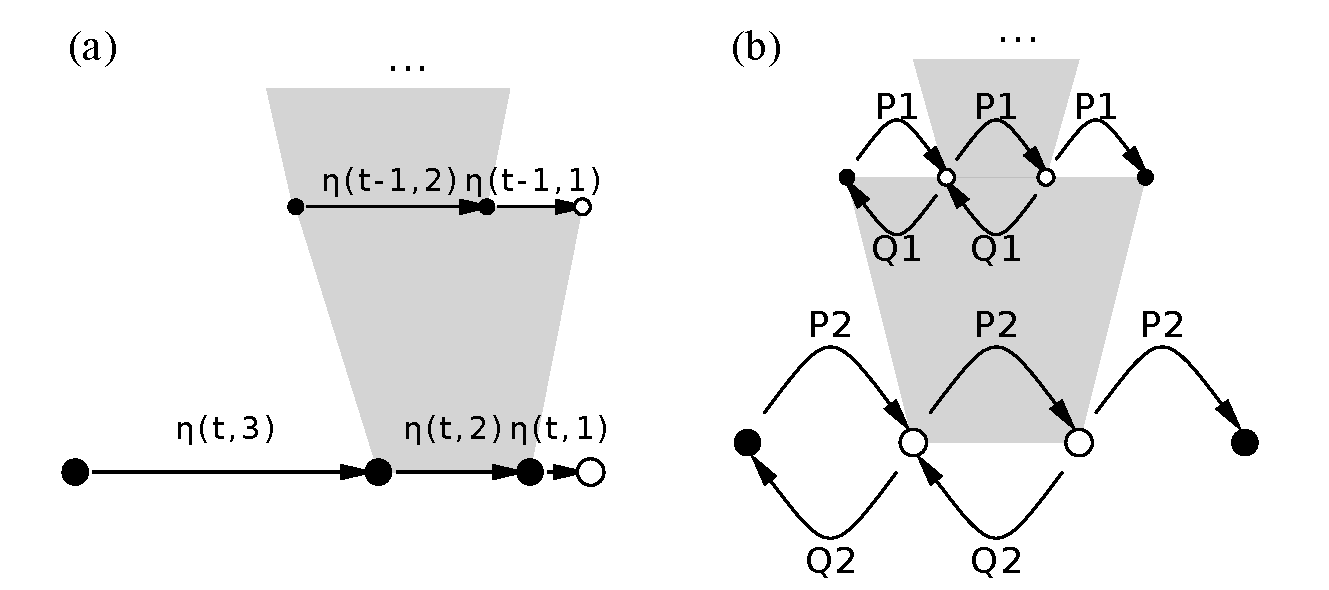
\includegraphics[width=0.88\columnwidth,trim={0 0cm 0 0cm},clip]{tradeoff.pdf}}
    \caption{(a) Treeverse algorithm for optimal checkpointing.~\cite{Griewank1992} $\eta(\tau, \delta) \equiv \left(\begin{matrix} \tau + \delta \\ \delta \end{matrix}\right)=\frac{(\tau+\delta)!}{\tau!\delta!}$ is the binomial function. (b) Bennett's time space trade-off scheme for reverse computing.~\cite{Bennett1973,Levine1990} $P$ and $Q$ are computing and uncomputing respectively. The pseudo-code is defined in \Lst{lst:bennett}.}\label{fig:tradeoff}
\end{figure}

\begin{minipage}{.88\columnwidth}
    \begin{lstlisting}[mathescape=true,caption={The Bennett's time-space trade-off scheme. Its NiLang implementation is in \App{app:bennett-nilang}.},label={lst:bennett}]
bennett($\{s_1,...\}$, k, i, len)
    if len == 1
        $s_{i+1}$ ← 0
        $f_i$($s_{i+1}$, $s_i$)
    else
        # P process that calls the forward program k steps
        bennett($\{s_1,...\}$, k, i+len÷k*(j-1), len÷k) for j=1,2,...,k
        # Q process that calls the backward program k-1 steps
        ~bennett($\{s_1,...\}$, k, i+len÷k*(j-1), len÷k) for j=k-1,k-2,...,1
\end{lstlisting}
\end{minipage}

The reverse computing does not show any advantage in worse-case complexity comparing with checkpointing.
But the following traits make it perform better in many practical applications.
\textit{First}, reverse computing can make use of the reversibility to save memory. The above discussion assumes every operation is irreversible, however, the most program contains a lot of reversible instructions like the multiply-accumulate operation in many BLAS functions and sparse matrix functions. In \App{app:reversibility}, we show how to implement a unitary matrix multiplication without introducing overheads in space and time.
\textit{Second}, reverse computing does not allocate automatically for users, user can optimize the memory access patterns for their own devices like GPU.
\textit{Third}, reverse computing is compatible with effective codes, so that it fits better with modern languages. In \App{app:effectivecode}, we show how to manipulate inplace functions on arrays with NiLang.
\textit{Fourth}, reverse computing can utilize the existing compiler to optimize the code better because it does not automatically introduce global stack operations that harm the purity of functions.
\textit{Fifth}, reverse computing encourages the user to think reversibly. Reversible thinking can lead the user to a constant memory, constant time overhead implementation of chained multiplication algorithms as shown in \App{app:chainedmul}.
Transpiling a regular code to a reversible code is not hard, but it is unlikely to provide the user with better performance than optimal checkpointing. Instead, thinking about how to write instructions and control flows reversibly does.

\section{Language design}\label{sec:lang}

NiLang is an embedded domain-specific language (eDSL) NiLang built on top of the host language Julia~\cite{Bezanson2012,Bezanson2017}.
Julia is a popular language for scientific programming and machine learning. We choose Julia mainly for speed. Julia is a language with high abstraction, however, its clever design of type inference and just in time compiling make it has a C like speed.
Meanwhile, it has rich features for meta-programming. Its package for pattern matching \href{https://github.com/thautwarm/MLStyle.jl}{MLStyle} allows us to define an eDSL in less than 2000 lines.
Comparing with a regular reversible programming language, NiLang features array operations, rich number systems including floating-point numbers, complex numbers, fixed-point numbers, and logarithmic numbers.
It also implements the compute-copy-uncompute~\cite{Bennett1973} macro to increase code reusability.
Besides the above reversible hardware compatible features, it also has some reversible hardware incompatible features to meet the practical needs. For example, it views the floating-point $\mathrel{+}$ and $\mathrel{-}$ operations as reversible. It also allows users to extend instruction sets and sometimes inserting external statements. These features are not compatible with future reversible hardware.
NiLang's source code is available online, we will put a link here after the anonymous open review session.
%\href{https://github.com/GiggleLiu/NiLang.jl}{https://github.com/GiggleLiu/NiLang.jl}, \href{https://github.com/GiggleLiu/NiLangCore.jl}{https://github.com/GiggleLiu/NiLangCore.jl}.
By the time of writing, the version of NiLang is v0.7.3.

\subsection{Reversible functions and instructions}
    Mathematically, any irreversible mapping \texttt{y = f(args...)} can be trivially transformed to its reversible form \texttt{y += f(args...)} or \texttt{y $\veebar$= f(args...)} ($\veebar$ is the bit-wise \texttt{XOR}), where \texttt{y} is a pre-emptied variable. But in numeric computing with finite precision, this is not always true. The reversibility of arithmetic instruction is closely related to the number system.
    For integer and fixed point number system, \texttt{y += f(args...)} and \texttt{y -= f(args...)} are rigorously reversible. For logarithmic number system and tropical number system~\cite{Speyer2009}, \texttt{y *= f(args...)} and \texttt{y /= f(args...)} as reversible (not introducing the zero element). While for floating point numbers, none of the above operations are rigorously reversible.
    However, for convenience, we ignore the round-off errors in floating-point \texttt{+} and \texttt{-} operations and treat them on equal footing with fixed-point numbers in the following discussion. In \App{app:roundoff}, we will show doing this is safe in most cases provided careful implementation.
Other reversible operations includes \texttt{SWAP}, \texttt{ROT}, \texttt{NEG} et. al., and this instruction set is extensible.
One can define a reversible multiplier in NiLang as in \Lst{lst:multiplier}.

\begin{minipage}{.88\columnwidth}
\begin{lstlisting}[mathescape=true,caption={A reversible multiplier},label={lst:multiplier}]
julia> using NiLang

julia> @i function multiplier(y!::Real, a::Real, b::Real)
           y! += a * b
       end

julia> multiplier(2, 3, 5)
(17, 3, 5)

julia> (~multiplier)(17, 3, 5)
(2, 3, 5)
\end{lstlisting}
\end{minipage}

Macro \texttt{@i} generates two functions that are reversible to each other, \texttt{multiplier} and \texttt{$\sim$multiplier}, each defines a mapping $\mathbb{R}^3 \rightarrow \mathbb{R}^3$. The $!$ after a symbol is a part of the name, as a conversion to indicate the mutated variables.

\subsection{Reversible memory management}
A distinct feature of reversible memory management is that the content of a variable must be known when it is deallocated.
We denote the allocation of a pre-emptied memory as \texttt{x $\leftarrow$ 0}, and its inverse, deallocating a \textbf{zero emptied} variable, as \texttt{x $\rightarrow$ 0}.
An unknown variable can not be deallocate, but can be pushed to a stack pop out later in the uncomputing stage.
If a variable is allocated and deallocated in the local scope, we call it an ancilla.
\Lst{lst:complex} defines the complex valued accumulative log function.

\begin{minipage}{.45\columnwidth}
\begin{lstlisting}[mathescape=true,caption={Reversible complex valued log function $y\mathrel{+}=\log(|x|) + i{\rm Arg}(x)$.},label={lst:complex}]
@i @inline function (:+=)(log)(y!::Complex{T}, x::Complex{T}) where T
    n ← zero(T)
    n += abs(x)

    y!.re += log(n)
    y!.im += angle(x)

    n -= abs(x)
    n → zero(T)
end
\end{lstlisting}
\end{minipage}\hfill
\begin{minipage}{.45\columnwidth}
    \begin{lstlisting}[mathescape=true,caption={Compute-copy-uncompute version of \Lst{lst:complex}},label={lst:complex2}]
@i @inline function (:+=)(log)(y!::Complex{T}, x::Complex{T}) where T
    @routine begin
        n ← zero(T)
        n += abs(x)
    end
    y!.re += log(n)
    y!.im += angle(x)
    ~@routine
end
\end{lstlisting}
\end{minipage}

Here, the macro \texttt{@inline} tells the compiler that this function can be inlined. One can input ``$\leftarrow$'' and ``$\rightarrow$'' by typing ``$\backslash$leftarrow[TAB KEY]'' and ``$\backslash$rightarrow[TAB KEY]'' respectively in a Julia editor or REPL.
NiLang does not have immutable structs, so that the real part \texttt{y!.re} and imaginary \texttt{y!.im} of a complex number can be changed directly.
It is easy to verify that the bottom two lines in the function body are the inverse of the top two lines. i.e., the bottom two lines \textit{uncomputes} the top two lines.
The motivation of uncomputing is to zero clear the contents in ancilla \texttt{n} so that it can be deallocated correctly.
\textit{Compute-copy-uncompute} is a useful design pattern in reversible programming so that we created a pair of macros \texttt{@routine} and \texttt{$\sim$@routine} for it. One can rewrite the above function as in \Lst{lst:complex2}.

\subsection{Reversible control flows}
One can define reversible \texttt{if}, \texttt{for} and \texttt{while} statements in a reversible program.
\Fig{fig:controlflow} (a) shows the flow chart of executing the reversible \texttt{if} statement. There are two condition expressions in this chart, a precondition and a postcondition. The precondition decides which branch to enter in the forward execution, while the postcondition decides which branch to enter in the backward execution. The pseudo-code for the forward and backward passes are shown in \Lst{lst:reversibleif1} and \Lst{lst:reversibleif2}.

\begin{minipage}{.45\columnwidth}
\begin{lstlisting}[mathescape=true,caption={Translating a reversible \texttt{if} statement (forward)},label={lst:reversibleif1}]
branchkeeper = precondition
if precondition
    branch A
else
    branch B
end
assert branchkeeper ==  postcondition
\end{lstlisting}
\end{minipage}
\hfill
\begin{minipage}{.45\columnwidth}
\begin{lstlisting}[mathescape=true,caption={Translating a reversible \texttt{if} statement (backward)},label={lst:reversibleif2}]
branchkeeper = postcondition
if postcondition
    ~(branch A)
else
    ~(branch B)
end
assert branchkeeper ==  precondition
\end{lstlisting}
\end{minipage}

\Fig{fig:controlflow} (b) shows the flow chart of the reversible \texttt{while} statement. It also has two condition expressions. Before executing the condition expressions, the program presumes the postcondition is false.
After each iteration, the program asserts the postcondition to be true. To reverse this statement, one can exchange the precondition and postcondition, and reverse the body statements. The pseudo-code for the forward and backward passes are shown in \Lst{lst:reversiblewhile1} and \Lst{lst:reversiblewhile2}.

\begin{minipage}{.45\columnwidth}
\begin{lstlisting}[mathescape=true,caption={Translating a reversible \texttt{while} statement (forward)},label={lst:reversiblewhile1}]
assert postcondition == false
while precondition
    loop body
    assert postcondition == true
end
\end{lstlisting}
\end{minipage}
\hfill
\begin{minipage}{.45\columnwidth}
\begin{lstlisting}[mathescape=true,caption={Translating a reversible \texttt{while} statement (backward)},label={lst:reversiblewhile2}]
assert precondition == false
while postcondition
    ~(loop body)
    assert precondition == true
end
\end{lstlisting}
\end{minipage}

The reversible \texttt{for} statement is similar to the irreversible one except that after execution, the program will assert the iterator to be unchanged. To reverse this statement, one can exchange \texttt{start} and \texttt{stop} and inverse the sign of \texttt{step}.
\begin{figure}
    \centerline{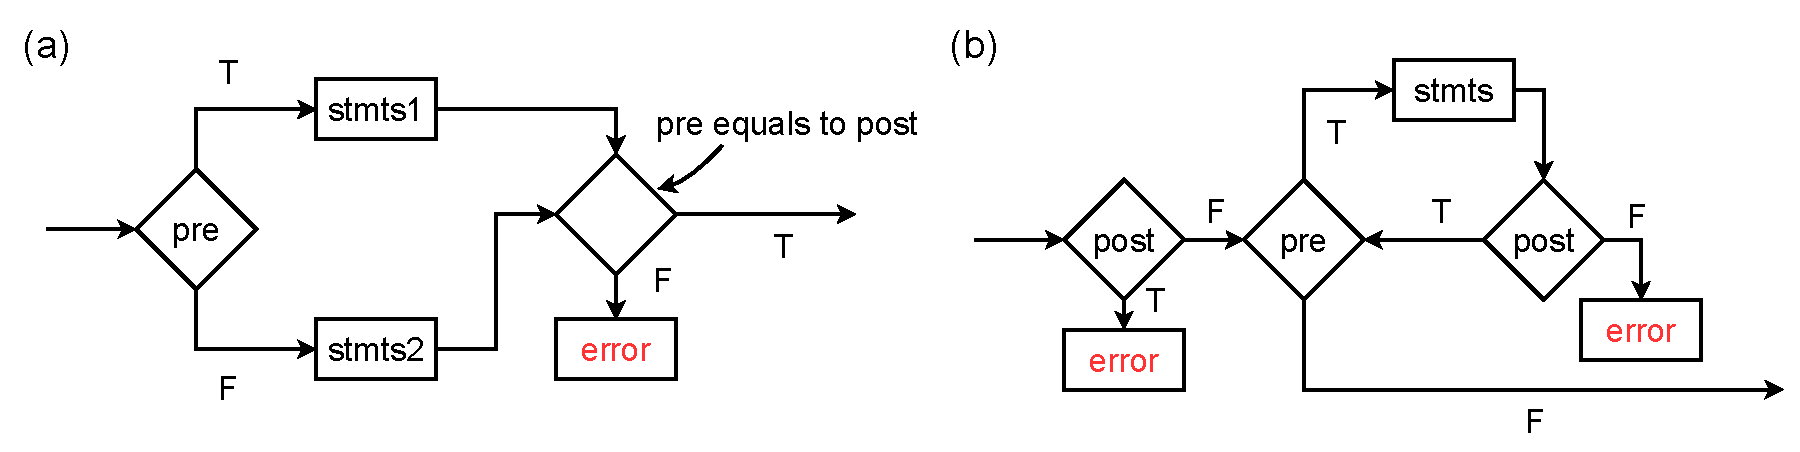
\includegraphics[width=0.9\columnwidth,trim={0 0cm 0 0cm},clip]{controlflow.pdf}}
    \caption{The flow chart for reversible (a) \texttt{if} statement and (b) \texttt{while} statement. ``pre'' and ``post'' represents precondition and postcondition respectively. The assersion errors are thrown to the host language instead of handling them in NiLang.}\label{fig:controlflow}
\end{figure}
\Lst{lst:fib} computes the Fibonacci number recursively and reversibly.

\begin{minipage}{.88\columnwidth}
\begin{lstlisting}[mathescape=true,caption={Computing Fibonacci number recursively and reversibly.},label={lst:fib}]
@i function rrfib(out!, n)
    @invcheckoff if (n >= 1, ~)
        counter ← 0
        counter += n
        while (counter > 1, counter!=n)
            rrfib(out!, counter-1)
            counter -= 2
        end
        counter -= n % 2
        counter → 0
    end
    out! += 1
end
\end{lstlisting}
\end{minipage}

Here, \texttt{out!} is an integer initialized to \texttt{0} for storing outputs.
The precondition and postcondition are wrapped into a tuple. In the \texttt{if} statement, the postcondition is the same as the precondition, hence we omit the postcondition by inserting a "\texttt{$\sim$}" in the second field for ``copying the precondition in this field as the postcondition''.
In the while statement, the postcondition is true only for the initial loop.
Once code is proven correct, one can turn off the reversibility check by adding \texttt{@invcheckoff} before a statement.
This will remove the reversibility check and make the code faster and compatible with GPU kernels (kernel functions can not handle exceptions).

\section{Reversible automatic differentiation}\label{sec:bp}

\subsection{Back propagation}
\begin{figure}[h!]
    \centerline{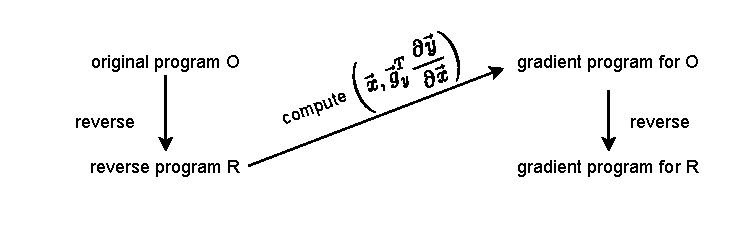
\includegraphics[width=0.8\columnwidth,trim={0 0cm 0 0},clip]{autodiff.pdf}}
    %\caption{Automatic differentiation.}\label{fig:autodiff}
\end{figure}
We decompose the problem of reverse mode AD into two sub-problems, \textbf{reversing the code} and \textbf{computing} $\frac{\partial \text{[single input]}}{\partial \text{[multiple outputs]}}$.
Reversing the code is trivial in reversible programming, while the second sub-problem is similar to forward mode automatic differentiation that computes $\frac{\partial \text{[multiple outputs]}}{\partial \text{[single input]}}$.
Inspired by the Julia package ForwardDiff~\cite{Revels2016}, we use operator overloading rather than the source to source transformation for better extensibility.
We wrap each output variable with a composite type \texttt{GVar} that containing an extra gradient field, and feed it into the reversed generic program.
Instructions are multiple dispatched to corresponding gradient instructions that update the gradient field of \texttt{GVar} at the same time. By reversing this gradient program, we can obtain the gradient program for the reversed program $R$ too.
One can define the adjoint (``adjoint'' here means a reversed program updating gradients) of a primitive instruction as a reversible function on \textbf{either} the function itself or its reverse since the adjoint of a function's reverse is equivalent to the reverse of the function's adjoint.
\begin{align}
    f: (\vec x, \vec g_x) &\rightarrow (\vec y, \vec g_x^T\frac{\partial \vec x}{\partial \vec y})\\
    f^{-1}: (\vec y, \vec g_y) &\rightarrow (\vec x, \vec g_y^T\frac{\partial \vec y}{\partial \vec x})
\end{align}
It can be easily verified by applying the above two mappings consecutively, which turns out to be an identity mapping considering $\frac{\partial \vec y}{\partial \vec x} \frac{\partial \vec x}{\partial \vec y} = \mathbbm{1}$.

The implementation details are described in \App{app:jacobian}.
In most languages, operator overloading brings significant overheads of function calls and object allocation and deallocation.
But in a language with type inference and just in time compiling like Julia, the boundary between two approaches are vague.
The compiler inlines small functions, packs an array of constant sized immutable objects into a continuous memory, and truncates unnecessary branches automatically.

\subsection{Hessians}
Combining forward mode AD and reverse mode AD is a simple yet efficient way to obtain Hessians.
By wrapping the elementary type with \texttt{Dual} defined in package ForwardDiff and throwing it into the gradient program defined in NiLang, one obtains one row/column of the Hessian matrix.
We will use this approach to compute Hessians in the graph embedding benchmark in \Sec{sec:graphbench}.

\subsection{CUDA kernels}
CUDA programming is playing a significant role in high-performance computing. In Julia, one can write GPU compatible functions in native Julia language with \href{https://github.com/JuliaGPU/KernelAbstractions.jl}{KernelAbstractions}.~\cite{Besard2018}
Since NiLang does not push variables into stack automatically for users, it is safe to write differentiable GPU kernels with NiLang.
We will differentiate CUDA kernels with no more than extra 10 lines in the bundle adjustment benchmark in \Sec{sec:benchmark}.

\section{Benchmarks}\label{sec:benchmark}

We benchmark our framework with the state-of-the-art GP-AD frameworks, including source code transformation based Tapenade and Zygote and operator overloading based ForwardDiff and ReverseDiff. 
Since most tensor based AD software like famous TensorFlow and PyTorch are not designed for the using cases used in our benchmarks, we do not include those package to avoid an unfair comparison.
In the following benchmarks, the CPU device is Intel(R) Xeon(R) Gold 6230 CPU @ 2.10GHz, and the GPU device is NVIDIA Titan V.
For NiLang benchmarks, we have turned the reversibility check off to achieve a better performance.

We reproduced the benchmarks for Gaussian mixture model (GMM) and bundle adjustment in ~\citet{Srajer2018} by re-writing the programs in a reversible style. We show the results in \Fig{fig:gmmba}. The Tapenade data is obtained by executing the docker file provided by the original benchmark, which provides a baseline for comparison.

\begin{figure}[h!]
    \centerline{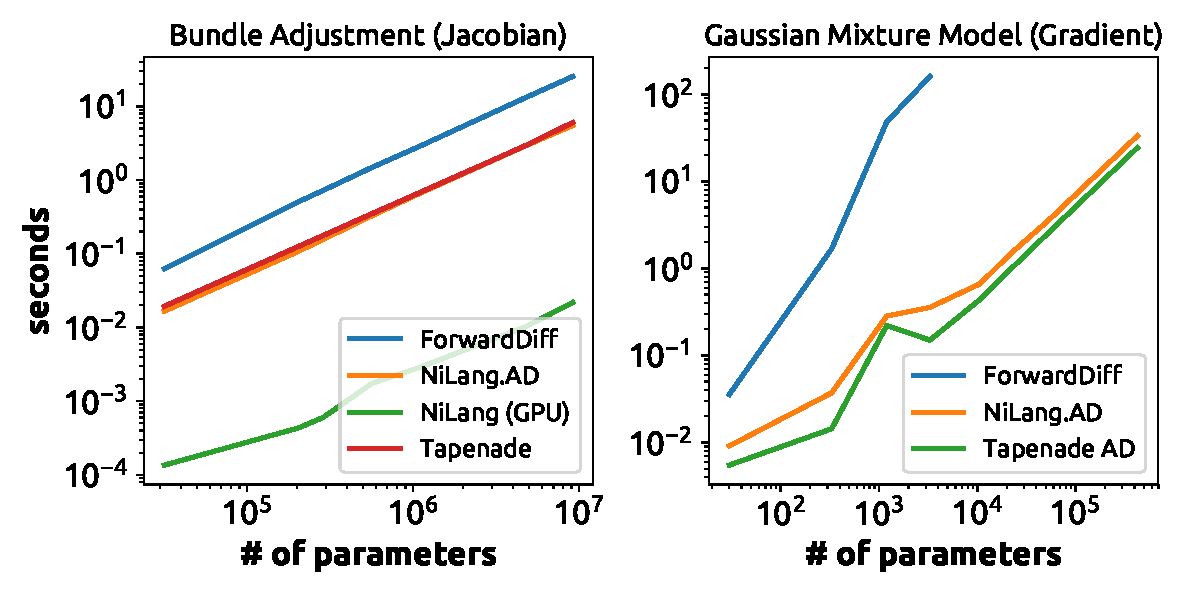
\includegraphics[width=0.95\columnwidth,trim={0 0cm 0 0},clip]{fig9.pdf}}
    \caption{Absolute runtimes in seconds for computing the objective (-O) and Jacobians (-J). (a) GMM with 10k data points, the loss function has a single output, hence computing Jacobian is the same as computing gradient. ForwardDiff data is missing due to not finishing in limited time. The NiLang GPU data is missing because we do not write kernel here. (b) Bundle adjustment.
    }\label{fig:gmmba}
\end{figure}

NiLang's objective function is $\sim 2\times$ slower than normal code due to the uncomputing overhead.
In this case, NiLang does not show advantage to Tapenade in obtaining gradients, the ratio between computing the gradients and the objective function are close.
This is because the bottleneck of this model is the matrix vector multiplication, traditional AD can already handle this function well.
The extra memory used to reverse the program is negligible comparing to the original program as shown in \Fig{fig:gmm-memory}.
The backward pass is not shown here, it is just two times the reversible program in order to store gradients. 
The data is obtained by counting the main memory allocations in the program manually. The analytical expression of memory usage in unit of floating point number is
\begin{align}
    S &= (2+d^2)k+2d + P, \\
    S_r &= (3+d^2+d)k+2{\log}_2k + P,
\end{align}
where $d$ and $k$ are the size and number of covariance matrices. $P = \frac{d(d+1)}{2}k + k + dk$ is the size of parameter space. The memory of the dataset ($d\times N$) is not included because it will scale as $N$.
Due to the hardness of estimating peak memory usage, the Tapenade data is missing here. The ForwardDiff memory usage is approximately the original size times the batch size, where the batch size is $12$ by default.
\begin{figure}
    \centerline{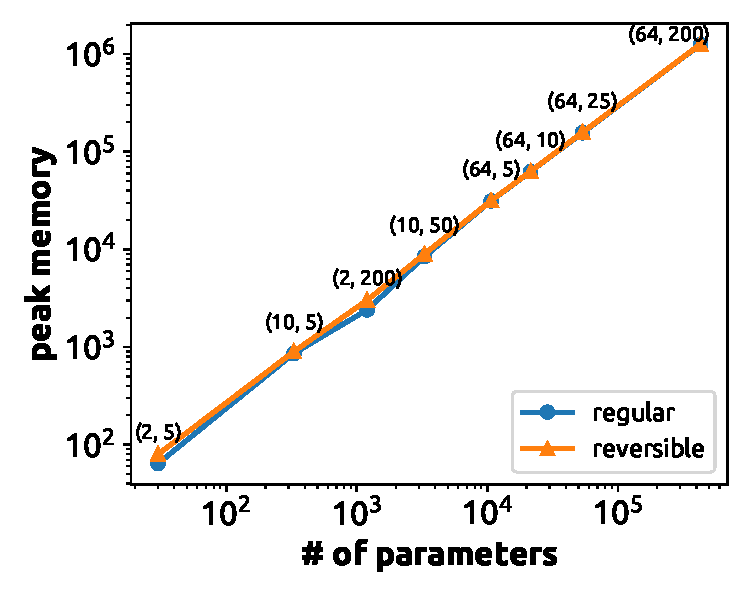
\includegraphics[width=0.55\columnwidth,trim={0 0cm 0 0},clip]{fig10.pdf}}
    \caption{Peak memory of running the original and the reversible GMM program. The labels are $(d, k)$ pairs.}\label{fig:gmm-memory}
\end{figure}

In the bundle adjustment benchmark, NiLang performs the best on CPU.
We also compiled our adjoint program to GPU with no more than 10 lines of code with KernelAbstractions, which provides another $\sim 200\times$ speed up.
Parallelizing the adjoint code requires the forward code not reading the same variable simultaneously in different threads, and this requirement is satisfied here.
The peak memory of the original program and the reversible program are both equal to the size of parameter space because all ``allocation''s happen on registers in this application.

One can find more benchmarks in \App{app:morebenchmarks}, including differentiating sparse matrix dot product and obtaining Hessians in the graph embedding application.

\section{Discussion}
In this work, we demonstrate a new approach to back propagates a program called reversible programming AD by designing a reversible eDSL NiLang.
NiLang is a powerful tool to differentiate code from the source code level so that can be directly useful to machine learning researches. It can generate efficient backward rules, which is exemplified in \App{app:zygote}.
It can also be used to differentiate reversible neural networks like normalizing flows~\cite{Kobyzev2019} to save memory, e.g. back-propagating NICE network~\cite{Dinh2014} with only constant space overheads.
Except for the above immediate benefits to the machine learning ecosystem, we also want to emphasize the broader impact of AD on reverse computing.
AD on reverse computing is related to two of the central issues limiting many machine learning applications. One is how to overcome the memory wall that has been extensively discussed in the main text, and another is how to reduce energy consumption.
AD on reverse computing provides a software stack that connecting machine learning with further technologies to save energy.

\subsubsection*{Acknowledgments}
The authors are grateful to the people who help improve this work and fundings that sponsored the research. To meet the anonymous criteria, we will add the acknowledgments after the open review session.
%Jinguo Liu thanks Lei Wang for motivating the project with possible applications to reversible integrator, normalizing flow, and neural ODE.
%Johann-Tobias Schäg for deepening the discussion about reversible programming with his mathematicians head.
%Marisa Kiresame and Xiu-Zhe Luo for discussion on the implementation details of source-to-source automatic differentiation,
%Shuo-Hui Li and Xun Gao for helpful discussion on differential geometry, Tong Liu and An-Qi Chen for helpful discussion on quantum adders and multipliers, Ying-Bo Ma for correcting typos by submitting pull requests, Chris Rackauckas for helpful discussion on reversible integrator, Mike Innes for reviewing the comments about Zygote, Jun Takahashi for discussion about the graph embedding problem, Simon Byrne and Chen Zhao for helpful discussion on floating-point and logarithmic numbers.
%The authors are supported by the National Natural Science Foundation of China under Grant No.~11774398, the Strategic Priority Research Program of Chinese Academy of Sciences Grant No.~XDB28000000.

\bibliographystyle{iclr2021_conference}
\bibliography{invc}

\appendix

\section{NiLang implementation of Bennett's time-space trade-off algorithm}\label{app:bennett-nilang}
\begin{minipage}{.88\columnwidth}
    \begin{lstlisting}[mathescape=true,caption={NiLang implementation of the Bennett's time-space trade-off scheme.},label={lst:bennett-nilang}]
using NiLang, Test

PROG_COUNTER = Ref(0)   # (2k-1)^n
PEAK_MEM = Ref(0)       # n*(k-1)+2

@i function bennett(f::AbstractVector, state::Dict{Int,T}, k::Int, base, len) where T
    if (len == 1, ~)
        state[base+1] ← zero(T)
        f[base](state[base+1], state[base])
        @safe PROG_COUNTER[] += 1
        @safe (length(state) > PEAK_MEM[] && (PEAK_MEM[] = length(state)))
    else
        n ← 0
        n += len÷k
        # the P process
        for j=1:k
            bennett(f, state, k, base+n*(j-1), n)
        end
        # the Q process
        for j=k-1:-1:1
            ~bennett(f, state, k, base+n*(j-1), n)
        end
        n -= len÷k
        n → 0
    end
end

k = 4
n = 4
N = k ^ n
state = Dict(1=>1.0)
f(x) = x * 2.0
instructions = fill(PlusEq(f), N)

# run the program
@instr bennett(instructions, state, k, 1, N)

@test state[N+1] $\approx$ 2.0^N && length(state) == 2
@test PEAK_MEM[] == n*(k-1) + 2
@test PROG_COUNTER[] == (2*k-1)^n
\end{lstlisting}
\end{minipage}

The input \texttt{f} is a vector of functions and \texttt{state} is a dictionary.
We also added some irreversible external statements (those marked with \texttt{@safe}) to help analyse to program.

\section{Cases where reverse computing shows advantage}\label{app:rev-advantages}
\subsection{Handling effective codes}\label{app:effectivecode}
Reverse computing can handling effective codes with mutable structures and arrays.
For example, the affine transformation can be implemented without any overhead.

\begin{minipage}{.88\columnwidth}
\begin{lstlisting}[mathescape=true,caption={Inplace affine transformation.},label={lst:affine}]
@i function i_affine!(y!::AbstractVector{T}, W::AbstractMatrix{T}, b::AbstractVector{T}, x::AbstractVector{T}) where T
    @safe @assert size(W) == (length(y!), length(x)) && length(b) == length(y!)
    @invcheckoff for j=1:size(W, 2)
        for i=1:size(W, 1)
            @inbounds y![i] += W[i,j]*x[j]
        end
    end
    @invcheckoff for i=1:size(W, 1)
        @inbounds y![i] += b[i]
    end
end
\end{lstlisting}
\end{minipage}

Here, the expression following the \texttt{@safe} macro is an external irreversible statement.

\subsection{Utilizing reversibility}\label{app:reversibility}
Reverse computing can utilize reversibility to trace back states without extra memory cost.
For example, we can define the unitary matrix multiplication that can be used in a type of memory-efficient recurrent neural network.~\cite{Jing2016}

\begin{minipage}{.88\columnwidth}
\begin{lstlisting}[mathescape=true,caption={Two level decomposition of a unitary matrix.},label={lst:affine}]
@i function i_umm!(x!::AbstractArray, θ)
    M ← size(x!, 1)
    N ← size(x!, 2)
    k ← 0
    @safe @assert length(θ) == M*(M-1)/2
    for l = 1:N
        for j=1:M
            for i=M-1:-1:j
                INC(k)
                ROT(x![i,l], x![i+1,l], θ[k])
            end
        end
    end
    k → length(θ)
end
\end{lstlisting}
\end{minipage}

\subsection{Encourages reversible thinking}\label{app:chainedmul}
Last but not least, reversible programming encourages users to code in a memory friendly style.
Since allocations in reversible programming are explicit, programmers have the flexibility to control how to allocate memory and which number system to use.
For example, to compute the power of a positive fixed-point number and an integer, one can easily write irreversible code as in \Lst{lst:power1}

\begin{minipage}{.45\columnwidth}
\begin{lstlisting}[mathescape=true,caption={A regular power function.},label={lst:power1}]
function mypower(x::T, n::Int) where T
    y = one(T)
    for i=1:n
        y *= x
    end
    return y
end
\end{lstlisting}
\end{minipage}\hfill
\begin{minipage}{.45\columnwidth}
\begin{lstlisting}[mathescape=true,caption={A reversible power function.},label={lst:power2}]
@i function mypower(out,x::T,n::Int) where T
    if (x != 0, ~)
        @routine begin
            ly ← one(ULogarithmic{T})
            lx ← one(ULogarithmic{T})
            lx *= convert(x)
            for i=1:n
                ly *= x
            end
        end
        out += convert(ly)
        ~@routine
    end
end
\end{lstlisting}
\end{minipage}

Since the fixed-point number is not reversible under \texttt{*=}, naive checkpointing would require stack operations inside a loop. With reversible thinking, we can convert the fixed-point number to logarithmic numbers to utilize the reversibility of \texttt{*=} as shown in \Lst{lst:power2}. Here, the algorithm to convert a regular fixed-point number to a logarithmic number can be efficient.~\cite{Turner2010}

\section{Implementation of AD in NiLang}\label{app:jacobian}
To backpropagate the program, we first reverse the code through source code transformation and then insert the gradient code through operator overloading.
If we inline all the functions in \Lst{lst:complex2}, the function body would be like \Lst{lst:expand-complex}.
The automatically generated inverse program (i.e. $(y, x) \rightarrow (y-\log(x), x)$) would be like \Lst{lst:reversed-complex}.

\begin{minipage}{.45\textwidth}
\begin{lstlisting}[mathescape=true,caption={The inlined function body of \Lst{lst:complex2}.},label={lst:expand-complex}, frame=tlrb]
@routine begin
    nsq ← zero(T)
    n ← zero(T)
    nsq += x[i].re ^ 2
    nsq += x[i].im ^ 2
    n += sqrt(nsq)
end
y![i].re += log(n)
y![i].im += atan(x[i].im, x[i].re)
~@routine
\end{lstlisting}
\end{minipage}\hfill
\begin{minipage}{.45\textwidth}
    \begin{lstlisting}[mathescape=true,caption={The inverse of \Lst{lst:expand-complex}.},label={lst:reversed-complex}, frame=tlrb]
@routine begin
    nsq ← zero(T)
    n ← zero(T)
    nsq += x[i].re ^ 2
    nsq += x[i].im ^ 2
    n += sqrt(nsq)
end
y![i].re -= log(n)
y![i].im -= atan(x[i].im, x[i].re)
~@routine
\end{lstlisting}
\end{minipage}

To compute the adjoint of the computational process in \Lst{lst:expand-complex}, one simply insert the gradient code into its inverse in \Lst{lst:reversed-complex}.
The resulting inlined code is show in \Lst{lst:grad-complex}.

\begin{minipage}{.88\columnwidth}
\listingcaption{Insert the gradient code into \Lst{lst:reversed-complex}, the original computational processes are highlighted in yellow background.}\label{lst:grad-complex}
\begin{lstlisting}[mathescape=true,label={lst:grad-complex}, multicols=2]
@routine begin
   nsq ← zero(GVar{T,T})
   n ← zero(GVar{T,T})

   gsqa ← zero(T)
   gsqa += x[i].re.x * 2
   x[i].re.g -= gsqa * nsq.g
   gsqa -= nsq.x * 2
   gsqa -= x[i].re.x * 2
   gsqa → zero(T)
   $\text{\colorbox{yellow}{nsq.x += x[i].re.x \textasciicircum 2}} $

   gsqb ← zero(T)
   gsqb += x[i].im.x * 2
   x[i].im.g -= gsqb * nsq.g
   gsqb -= x[i].im.x * 2
   gsqb → zero(T)
   $\text{\colorbox{yellow}{nsq.x += x[i].im.x \textasciicircum 2}} $

   @zeros T ra rb
   rta += sqrt(nsq.x)
   rb += 2 * ra
   nsq.g -= n.g / rb
   rb -= 2 * ra
   ra -= sqrt(nsq.x)
   ~@zeros T ra rb
   $\text{\colorbox{yellow}{n.x += sqrt(nsq.x)}} $
end

$\text{\colorbox{yellow}{y![i].re.x -= log(n.x)}} $
n.g += y![i].re.g / n.x

$\text{\colorbox{yellow}{y![i].im.x-=atan(x[i].im.x,x[i].re.x)}} $
@zeros T xy2 jac_x jac_y
xy2 += abs2(x[i].re.x)
xy2 += abs2(x[i].im.x)
jac_y += x[i].re.x / xy2
jac_x += (-x[i].im.x) / xy2
x[i].im.g += y![i].im.g * jac_y
x[i].re.g += y![i].im.g * jac_x
jac_x -= (-x[i].im.x) / xy2
jac_y -= x[i].re.x / xy2
xy2 -= abs2(x[i].im.x)
xy2 -= abs2(x[i].re.x)
~@zeros T xy2 jac_x jac_y

~@routine
\end{lstlisting}
\end{minipage}

Here, \texttt{@zeros TYPE var1 var2...} is the macro to allocate multiple variables of the same type. Its inverse operations starts with \texttt{$\sim$@zeros} deallocates zero emptied variables.
In practice, ``inserting gradients'' is not achieved by source code transformation, but by operator overloading. We change the element type to a composite type \texttt{GVar} with two fields, value \texttt{x} and gradient \texttt{g}.
With multiple dispatching primitive instructions on this new type, values and gradients can be updated simultaneously.
Although the code looks much longer, the computing time (with reversibility check closed) is not.

\begin{minipage}{.88\textwidth}
\begin{lstlisting}[mathescape=true,caption={Time and allocation to differentiate complex valued log.},label={lst:time-complex}, frame=tlrb]
julia> @inline function (ir_log)(x::Complex{T}) where T
           log(abs(x)) + im*angle(x)
       end

julia> @btime ir_log(x) setup=(x=1.0+1.2im); # native code
  30.097 ns (0 allocations: 0 bytes)

julia> @btime (@instr y += log(x)) setup=(x=1.0+1.2im; y=0.0+0.0im); # reversible code
  17.542 ns (0 allocations: 0 bytes)

julia> @btime (@instr ~(y += log(x))) setup=(x=GVar(1.0+1.2im, 0.0+0.0im); y=GVar(0.1+0.2im, 1.0+0.0im)); # adjoint code
  25.932 ns (0 allocations: 0 bytes)
\end{lstlisting}
\end{minipage}

The performance is unreasonably good because the generated Julia code is further compiled to LLVM so that it can enjoy existing optimization passes.
For example, the optimization passes can find out that for an irreversible device, uncomputing local variables \texttt{n} and \texttt{nsq} to zeros does not affect return values, so that it will ignore the uncomputing process automatically.
Unlike checkpointing based approaches that focus a lot in the optimization of data caching on a global stack, NiLang does not have any optimization pass in itself.
Instead, it throws itself to existing optimization passes in Julia. Without accessing the global stack, NiLang's code is quite friendly to optimization passes.
In this case, we also see the boundary between source code transformation and operator overloading can be vague in a Julia, in that the generated code can be very different from how it looks.

The joint functions for primitive instructions \texttt{(:+=)(sqrt)} and \texttt{(:-=)(sqrt)} used above can be defined as in \Lst{lst:sqrt}.

\begin{minipage}{.88\textwidth}
    \begin{lstlisting}[mathescape=true,caption={Adjoints for primitives \texttt{(:+=)(sqrt)} and \texttt{(:-=)(sqrt)}.},label={lst:sqrt}, frame=tlrb]
@i @inline function (:-=)(sqrt)(out!::GVar, x::GVar{T}) where T
    @routine @invcheckoff begin
        @zeros T a b
        a += sqrt(x.x)
        b += 2 * a
    end
    out!.x -= a
    x.g += out!.g / b
    ~@routine
end
\end{lstlisting}
\end{minipage}

\section{More Benchmarks}\label{app:morebenchmarks}
\subsection{Sparse matrices}\label{sec:benchsparse}
We benchmarked the call, uncall and backward propagation time used for sparse matrix dot product and matrix multiplication.
Here, we estimate the time for back propagating gradients rather than including both forward and backward, since \texttt{mul!} does not output a scalar as loss.

\begin{table}[h!]\centering
\begin{minipage}{0.8\columnwidth}
\ra{1.3}
    \scalebox{1.0}{
        \begin{tabularx}{\textwidth}{bsb}\toprule
            \textbf{}     & \texttt{dot}         & \texttt{mul!} (complex valued) \\
            \hline
            Julia-O       & 3.493e-04   & 8.005e-05\\
            NiLang-O      & 4.675e-04   & 9.332e-05\\
            \hline
            NiLang-B      & 5.821e-04   & 2.214e-04\\
            \bottomrule
        \end{tabularx}
    }
    \caption{Absolute runtimes in seconds for computing the objectives (O) and the backward pass (B) of sparse matrix operations. The matrix size is $1000 \times 1000$, and the element density is $0.05$. The total time used in computing gradient can be estimated by summing ``O'' and ``B''.
    }\label{tbl:sparse}
\end{minipage}
\end{table}

The time used for computing backward pass is approximately 1.5-3 times the Julia's native forward pass.
This is because the instruction length of differentiating basic arithmetic instructions is longer than pure computing.


\subsection{Graph embedding problem}\label{sec:graphbench}
Graph embedding can be used to find a proper representation for an order parameter~\cite{Takahashi2020} in condensed matter physics. People want to find a minimum Euclidean space dimension $k$ that a Petersen graph can embed into, that the distances between pairs of connected vertices are $l_1$, and the distance between pairs of disconnected vertices are $l_2$, where $l_2 > l_1$.
The Petersen graph is shown in \Fig{fig:petersen}.
Let us denote the set of connected and disconnected vertex pairs as $L_1$ and $L_2$, respectively. This problem can be variationally solved with the following loss.
\begin{align}
    \begin{split}
        \mathcal{L} &= \Var({\rm dist}(L_1)) + \Var({\rm dist}(L_2)) \\
        &+\exp({\rm relu}(\overline{{\rm dist}(L_1)} - \overline{{\rm dist}(L_2)} + 0.1))) - 1
    \end{split}
\end{align}
The first line is a summation of distance variances in two sets of vertex pairs, where $\Var(X)$ is the variance of samples in $X$.
The second line is used to guarantee $l_2 > l_1$, where $\overline{X}$ means taking the average of samples in $X$.
Its reversible implementation could be found in our benchmark repository.

We repeat the training for dimension $k$ from $1$ to $10$.
In each training, we fix two of the vertices and optimize the positions of the rest. Otherwise, the program will find the trivial solution with overlapped vertices. 
For $k < 5$, the loss is always much higher than $0$,
while for $k\geq5$, we can get a loss close to machine precision with high probability.
From the $k=5$ solution, it is easy to see $l_2/l_1 = \sqrt{2}$.
An Adam optimizer with a learning rate $0.01$~\cite{Kingma2014} requires $\sim2000$ steps training.
The trust region Newton's method converges much faster, which requires $\sim 20$ computations of Hessians to reach convergence.
Although training time is comparable, the converged precision of the later is much better.
\begin{figure}
    \centerline{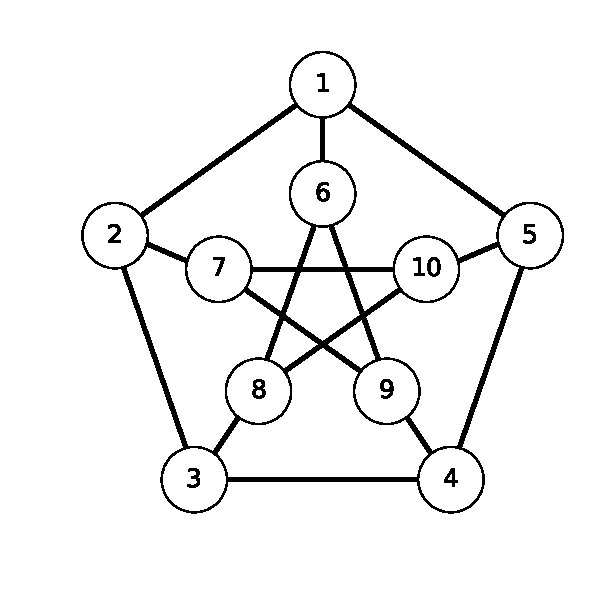
\includegraphics[width=0.4\columnwidth,trim={0 1cm 0 0},clip]{petersen.pdf}}
    \caption{The Petersen graph has 10 vertices and 15 edges. We want to find a minimum embedding dimension for it.}\label{fig:petersen}
\end{figure}

Since one can combine ForwardDiff and NiLang to obtain Hessians,
it is interesting to see how much performance we can get in differentiating the graph embedding program.

\begin{table}[h!]\centering
    \small
\begin{minipage}{\columnwidth}
\ra{1.3}
    \scalebox{1.0}{
        \begin{tabularx}{\textwidth}{bssssssssss}\toprule
            $k$                      & 2          & 4          & 6          & 8          & 10         \\
            \hline
            Julia-O                  & 4.477e-06  & 4.729e-06  & 4.959e-06  & 5.196e-06  & 5.567e-06  \\
            NiLang-O                 & 7.173e-06  & 7.783e-06  & 8.558e-06  & 9.212e-06  & 1.002e-05  \\
            NiLang-U                 & 7.453e-06  & 7.839e-06  & 8.464e-06  & 9.298e-06  & 1.054e-05  \\
            \hline
            NiLang-G                 & 1.509e-05  & 1.690e-05  & 1.872e-05  & 2.076e-05  & 2.266e-05  \\
            ReverseDiff-G            & 2.823e-05  & 4.582e-05  & 6.045e-05  & 7.651e-05  & 9.666e-05  \\
            ForwardDiff-G            & 1.518e-05  & 4.053e-05  & 6.732e-05  & 1.184e-04  & 1.701e-04  \\
            Zygote-G                 & 5.315e-04  & 5.570e-04  & 5.811e-04  & 6.096e-04  & 6.396e-04  \\
            \hline
            (NiLang+F)-H             & 4.528e-04  & 1.025e-03  & 1.740e-03  & 2.577e-03  & 3.558e-03  \\
            ForwardDiff-H            & 2.378e-04  & 2.380e-03  & 6.903e-03  & 1.967e-02  & 3.978e-02  \\
            (ReverseDiff+F)-H        & 1.966e-03  & 6.058e-03  & 1.225e-02  & 2.035e-02  & 3.140e-02  \\
            \bottomrule
        \end{tabularx}
    }
    \caption{Absolute times in seconds for computing the objectives (O), uncall objective (U), gradients (G) and Hessians (H) of the graph embedding program.
    $k$ is the embedding dimension, the number of parameters is $10k$.
    }\label{tbl:graphembedding}
\end{minipage}
\end{table}

In \Tbl{tbl:graphembedding}, we show the the performance of different implementations by varying the dimension $k$. The number of parameters is $10k$.
As the baseline, (a) shows the time for computing the function call. We have reversible and irreversible implementations, where the reversible program is slower than the irreversible native Julia program by a factor of $\sim2$ due to the uncomputing overhead.
The reversible program shows the advantage of obtaining gradients when the dimension $k \geq 3$. The larger the number of inputs, the more advantage it shows due to the overhead proportional to input size in forward mode AD.
The same reason applies to computing Hessians, where the combo of NiLang and ForwardDiff gives the best performance for $k \geq 3$.

\section{Porting NiLang to Zygote}\label{app:zygote}

Zygote is a popular machine learning package in Julia. We can port NiLang's automatically generated backward rules to Zygote to accelerate some performance-critical functions.
The following example shows how to speed up the backward propagation of \texttt{norm} by $\sim$50 times.

\begin{minipage}{.88\textwidth}
    \begin{lstlisting}[mathescape=true,caption={Porting NiLang to Zygote.},label={lst:zygote}, frame=tlrb]
julia> using Zygote, NiLang, NiLang.AD, BenchmarkTools, LinearAlgebra

julia> x = randn(1000);

julia> @benchmark norm'(x)
BenchmarkTools.Trial: 
  memory estimate:  339.02 KiB
  allocs estimate:  8083
  --------------
  minimum time:     228.967 μs (0.00% GC)
  median time:      237.579 μs (0.00% GC)
  mean time:        277.602 μs (12.06% GC)
  maximum time:     5.552 ms (94.00% GC)
  --------------
  samples:          10000
  evals/sample:     1

julia> @i function r_norm(out::T, out2::T, x::AbstractArray{T}) where T
          for i=1:length(x)
              @inbounds out2 += x[i]^2
          end
          out += sqrt(out2)
       end

julia> Zygote.@adjoint function norm(x::AbstractArray{T}) where T
          # compute the forward with regular norm (might be faster)
          out = norm(x)
          # compute the backward with NiLang's norm, element type is GVar
          out, δy -> (grad((~r_norm)(GVar(out, δy), GVar(out^2), GVar(x))[3]),)
       end

julia> @benchmark norm'(x)
BenchmarkTools.Trial: 
  memory estimate:  23.69 KiB
  allocs estimate:  2
  --------------
  minimum time:     4.015 μs (0.00% GC)
  median time:      5.171 μs (0.00% GC)
  mean time:        6.872 μs (13.00% GC)
  maximum time:     380.953 μs (93.90% GC)
  --------------
  samples:          10000
  evals/sample:     7
\end{lstlisting}
\end{minipage}

We first import the \texttt{norm} function from Julia standard library LinearAlgebra.
Zygote's builtin AD engine will generate a slow code and memory allocation of 339KB.
Then we write a reversible norm function \texttt{r\_norm} with NiLang and port the backward function to Zygote by specifying the backward rule (the function marked with macro \texttt{Zygote.@adjoint}).
Except for the speed up in computing time, the memory allocation also decreases to 23KB, which is equal to the sum of the original $x$ and the array used in backpropagation.
$$(1000\times 8 + 1000\times 8\times 2)/1024 \approx 23$$
The later one has a doubled size because \texttt{GVar} has an extra gradient field.

\section{A benchmark of round-off error in leapfrog}\label{app:roundoff}

%\begin{figure}
%    \centerline{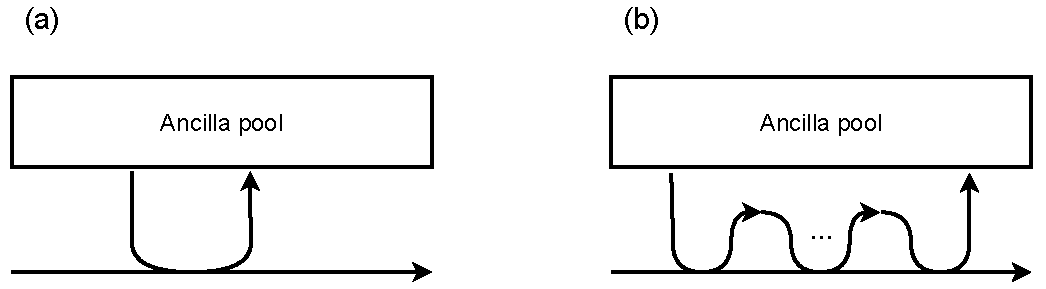
\includegraphics[width=0.7\columnwidth,trim={0 0cm 0 0},clip]{error.pdf}}
%    \caption{Two types of processes generating round off errors. (a) compute-uncompute on an ancilla for only once and then free it.
%    (b) Compute-uncompute on the same variable multiple times.}\label{fig:error}
%\end{figure}

\begin{figure}
    \centerline{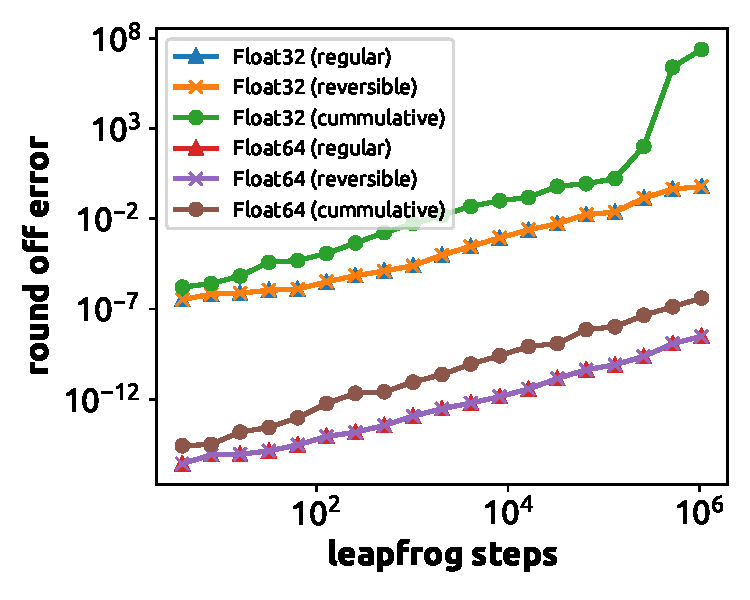
\includegraphics[width=0.5\columnwidth,trim={0 0cm 0 0},clip]{fig11.pdf}}
    \caption{Round-off errors in the final axes of planets as a function of the number of time steps. ``(regular)'' means an irreversible program, ``(reversible)'' means a reversible program (\Lst{lst:acc1}), and ``(ccumulative)'' means a reversible program with the acceleration computed with ccumulative errors (\Lst{lst:acc2}).}\label{fig:leapfrog}
\end{figure}
Running reversible programming with the floating pointing number system can introduce round-off errors and make the program not reversible. The quantify the effects, we use the leapfrog integrator to compute the orbitals of planets in our solar system as a benchmark. The leapfrog interations can be represented as
\begin{align}
    \vec a_i &= G\frac{m_j (\vec x_j-\vec x_i)}{\|\vec x_i - \vec x_j\|^3}\\
    \vec v_{i+1/2} &= \vec v_{i-1/2} + \vec a_{i} \Delta t\\
    \vec x_{i+1} &= \vec x_i + \vec v_{i+1/2}\Delta t
\end{align}
where $G$ is the gravitational constant and $m_j$ is the mass of $j$th planet, $\vec x$, $\vec v$ and $\vec a$ are location, velocity and acceleration respectively. The first value of velocity is $v_{1/2} = a_0 \Delta t/2$.
Since the dynamics of our solar system are symplectic and the leapfrog integrator is time-reversible, the reversible program does not have overheads and the evolution time can go arbitrarily long with constant memory.
We compare the mean error in the final axes of the planets and show the results in \Fig{fig:leapfrog}.
Errors are computed by comparing with the results computed with high precision floating-point numbers.
One of the key steps that introduce round-off error is the computation of \texttt{acceleration}. If it is implemented as in \Lst{lst:acc1}, the round-off error does not bring additional effect in the reversible context, hence we see overlapping lines ``(regular)'' and ``(reversible)'' in the figure.
This is because, when returning a dirty (not exactly zero cleared due to the floating-point round-off error) ancilla to the ancilla pool, the small remaining value will be zero-cleared automatically in NiLang.
The \texttt{acceleration} function can also be implemented as in \Lst{lst:acc2}, where the same variable \texttt{rb} is repeatedly used for compute and uncompute, the error will accumulate on this variable.
In both \texttt{Float64} (double precision floating point) and \texttt{Float32} (single precision floating point) benchmarks, the results show a much lower precision.
Hence, simulating reversible programming with floating-point numbers does not necessarily make the results less reliable if one can avoid cumulative errors in the implementation.

\begin{minipage}{.45\textwidth}
    \begin{lstlisting}[mathescape=true,caption={Compute the acceleration. Compute and uncompute on ancilla \texttt{rc}},label={lst:acc1}, frame=tlrb]
@i function :(+=)(acceleration)(y!::V3{T}, ra::V3{T}, rb::V3{T}, mb::Real, G) where T
    @routine @invcheckoff begin
        @zeros T d anc1 anc2 anc3 anc4
        rc ← zero(V3{T})
        d += sqdistance(ra, rb)
        anc1 += sqrt(d)
        anc2 += anc1 ^ 3
        anc3 += G * mb
        anc4 += anc3 / anc2
        rc += rb - ra
    end
    y! += anc4 * rc
    ~@routine
end
\end{lstlisting}
\end{minipage}
\hfill
\begin{minipage}{.45\textwidth}
    \begin{lstlisting}[mathescape=true,caption={Compute the acceleration. Compute and uncompute on the input variable \texttt{rb}.},label={lst:acc2}, frame=tlrb]
@i function :(+=)(acceleration)(y!::V3{T}, ra::V3{T}, rb::V3{T}, mb::Real, G) where T
    @routine @invcheckoff begin
        @zeros T d anc1 anc2 anc3 anc4
        d += sqdistance(ra, rb)
        anc1 += sqrt(d)
        anc2 += anc1 ^ 3
        anc3 += G * mb
        anc4 += anc3 / anc2
        rb -= ra
    end
    y! += anc4 * rb
    ~@routine
    # rb is not recovered rigorously!
end
\end{lstlisting}
\end{minipage}

\end{document}
